% COntinued Chpater Implementation
\section{Implementation Approaches}
\label{sec:impl_approaches}
\subsection{Content Based Model}
\label{sec:cb}

The content-based model uses Vector Space Models (VSM) of a user and an item to find the similarity between two vectors. The overview of content-based model is described in the \autoref{fig:content_based_flowchart} where all user interactions are denoted by \lq{}Users Ratings\rq{} and all recipes information is denoted by \lq{}Recipes\rq{}.
\begin{singlespace}
\begin{figure}[H]
	\centering
	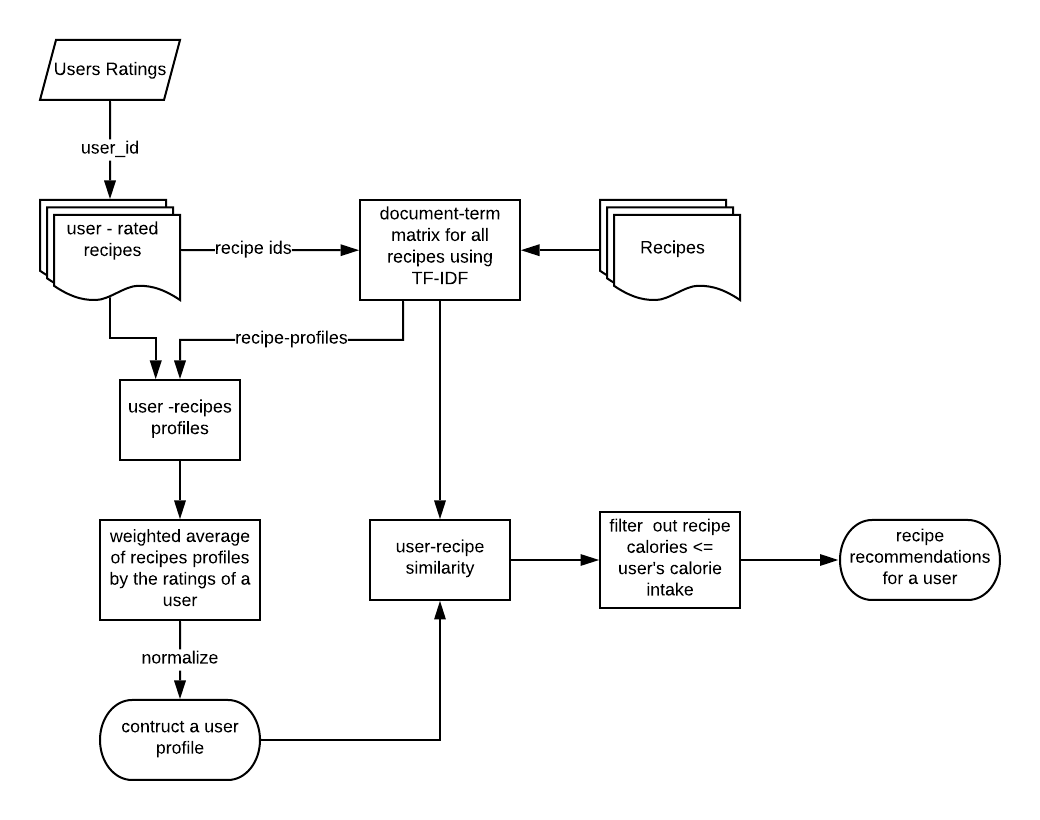
\includegraphics[width=1.0\linewidth]{content_based_flowchart}
	\caption{Content Based Filtering Work-Flow }
	\label{fig:content_based_flowchart}
\end{figure}  
\end{singlespace}

\noindent
Required steps to generated a user profile and a recipe profile in the flowchart are discussed below.
\begin{itemize}
\item All recipe profiles are generated based on the relevancy of terms to be considered. The term may vary based on the application area. In this thesis, ingredients, cooking methods, and diet labels are considered. The relevancy of terms in the documents is measured by TF-IDF as discussed in section \nameref{sec:tf-idf}. A document-term matrix is generated and stored for all recipes.
\item Rated recipes for a single user are filtered from all user interactions. Rated recipes are then filtered out from the document-term matrix.
\item To construct a user profile, recipes vectors rated by a user are considered. Then a weighted average of rated recipe profiles is calculated. The user profile is further normalized on the weighted values.
\item Similarity between the user profile and all recipe profiles from the dataset is measured by cosine similarity as discussed in section \nameref{cosine_similarity}. The system should not recommend the same recipes that are rated by a user previously. Hence, previously rated recipes by a user are omitted before calculating relevance. Remaining recipes are then sorted in descending order of similarity scores.
\item On the resultant recipes vectors, a calorie intake filter is applied, comparing recipe calories and user required calories. In calorie filter, the system considers only those recipes whose calories are less or equal to user\rq{}s calorie intake requirement. These recipes are offered as recommendations to the user.
\end{itemize}
 
\begin{singlespace}
\begin{figure}[H]
	\centering
	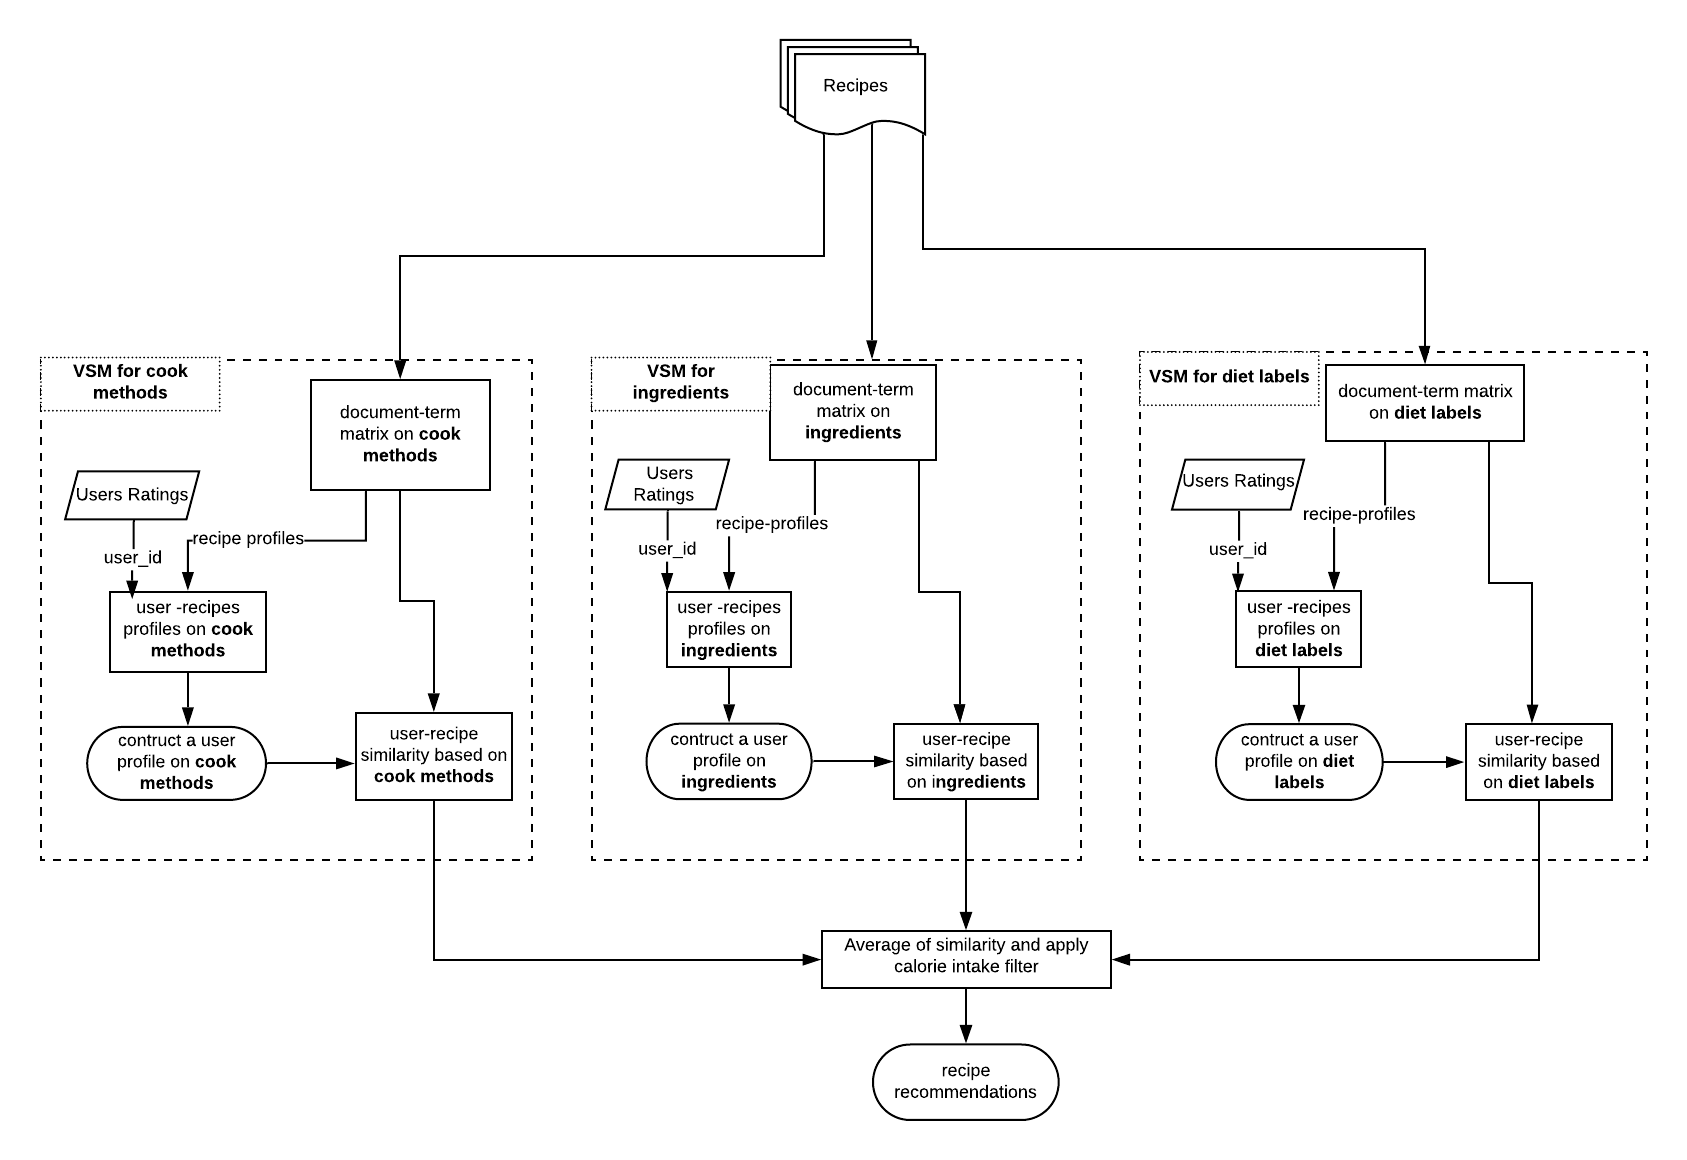
\includegraphics[width=1.0\linewidth]{content_based_ingredients_cookmethod_dietlabels}
	\caption{Content Based Filtering Combined Work-Flow }
	\label{fig:content_based_ingredients_cookmethod_dietlabels}
\end{figure}  
\end{singlespace}


\subsubsection{Content-Based Using Ingredients}
\label{sec:cb_ingredients}
Recipe ingredients are used to calculate recommendations in content-based using the ingredients approach. The user profile and recipe profiles are generated using ingredients in the recipes. The steps to generate recommendations for a user using ingredients in the content-based model are discussed below.\\
All ingredients from recipes are extracted. The similarity between recipes is considered based on ingredients but many ingredients occur in all recipes such as salt. To get the importance of ingredients that are relevant to the recipe and to negate the effect of high-frequency terms, the concept of TF-IDF has been used as discussed in section \nameref{sec:tf-idf}. The recipe vector or recipe profile is calculated for each recipe in the dataset. The \lq{}TfidfVectorizer\rq{} function from \lq{}sklearn\rq{} library has been used to calculate TF-IDF. The VSM for ingredients in the \autoref{fig:content_based_ingredients_cookmethod_dietlabels} represents Vector Space Model using ingredients. The weighted average of a user rated recipe profiles is calculated to construct a user profile. The similarity between a user profile and all recipe profiles in the dataset is calculated using cosine similarity. The \lq{}linear\_kernel\rq{} function from the \lq{}sci-kit learn\rq{} library has been used for the same. The resultant profiles are listed in descending order of similarity score to get more relevant recipes at the top. At this point recipes already rated by a user are omitted. From the user's information, the BMR and the required calorie intake per meal are calculated as discussed in section \nameref{sec:user_info}. The resultant set of recipes is offered as recommendations. 

\subsubsection{Content-Based Using Ingredients and Cook Methods}
\label{sec:cb_ingredients_cook_method}
Recipe ingredients and cook methods are used to calculate recommendations in content-based using ingredients and cook method approach. The extraction process of cook methods from cooking directions is discussed in section \nameref{sec:cook_method}.  The user profile and recipe profiles are generated using the cooking method in the recipes. The VSM for cook method in the \autoref{fig:content_based_ingredients_cookmethod_dietlabels} represents Vector Space Model using cook method. The recipe vector is calculated for each recipe in the dataset. The constructed user profile is based on cook methods of the recipes. The similarity between a user profile and all recipe profiles in the dataset is calculated using cosine similarity. Further, the average of cosine similarity scores generated using ingredients and cook methods is considered as a result. The resultant profiles are listed in descending order of similarity score to get more relevant recipes at the top. At this point recipes already rated by a user are omitted. From the user's information, the BMR and the required calorie intake per meal are calculated as discussed in section \nameref{sec:user_info}. The resultant set of recipes is offered as recommendations. 

\subsubsection{Content-Based Using Ingredients, Cook Methods and Diet Labels}
\label{sec:cb_ingredients_cook_method_diet_labels}
Recipe ingredients, cook methods and diet labels are used to calculate recommendations in content-based using ingredients, cook methods and diet labels approach. Extraction process of diet labels from nutrition attribute is discussed in the section \nameref{sec:diet_labels}. In addition to ingredients and cook methods, the user profile and recipe profiles are generated using diet labels in the recipes.. The VSM for diet labels in the \autoref{fig:content_based_ingredients_cookmethod_dietlabels} represents Vector Space Model using diet labels. The recipe vector is calculated for each recipe in the dataset. The constructed user profile is based on diet labels of the recipes. The similarity between a user profile and all recipe profiles in the dataset is calculated using cosine similarity. Further, the average of cosine similarity scores generated using ingredients, cook methods and diet labels is considered as a result. The resultant profiles are listed in descending order of similarity score to get more relevant recipes at the top. At this point recipes already rated by a user are omitted. From the user's information, the BMR and the required calorie intake per meal are calculated as discussed in section \nameref{sec:user_info}. The resultant set of recipes is offered as recommendations. 

\subsection{Collaborative Filtering Model}
\label{sec:cf}
Model-based collaborative filtering for the user and recipes was applied. This approach utilizes information related to user ratings on the recipes. A Singular Value Decomposition (SVD) algorithm has been applied to get the recommendations. The below approach was followed to get recommendations using SVD.
\begin{singlespace}
\begin{figure}[H]
\centering
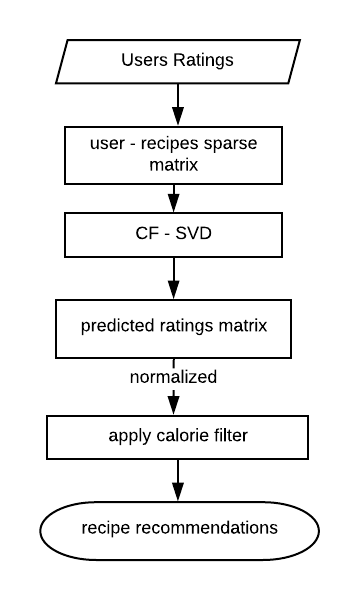
\includegraphics[width=0.5 \linewidth]{cf-svd}
\caption{Collaborative Filtering- SVD Work-Flow }
\label{fig:cf-svd}
\end{figure}
\end{singlespace}

\begin{itemize}
\item All user ids and recipe ids are extracted in such a way that every user id and recipe id represents a unique relationship via rating. The user id refers to unique id given to the user and recipe id refers to a unique id given to the recipe in the dataset. The matrix of user-recipes ratings is formed such as a user represents row and recipes represents columns. The cell value represents a rating for a recipe given by a user. From this matrix, the sparse matrix was created.
\item The sparse matrix is the same as the above matrix except it has high efficiency to perform large mathematical operations. To create a sparse matrix, 'csr\_matrix' function is used from 'scipy.sparse' library. The generated sparse matrix was sent as an input to the SVD algorithm.
\item SVD algorithm runs Principal Component Analysis (PCA) on the user-rating matrix to give back factors of the rating matrix as discussed in \nameref{sec:svd}. The dot product of these factors returns a rating matrix with predicted ratings.
\item Further, normalization was performed to get all predicted ratings for all users, for all recipes.
\end{itemize}

\subsection{Hybrid Model(CB and CF)}
\label{sec:hybrid_impl}
The hybrid model is a combination of content-based and collaborative filtering. The work-flow of the application using the hybrid technique is depicted in the \autoref{fig:hybrid}.
\begin{singlespace}
\begin{figure}[H]
\centering
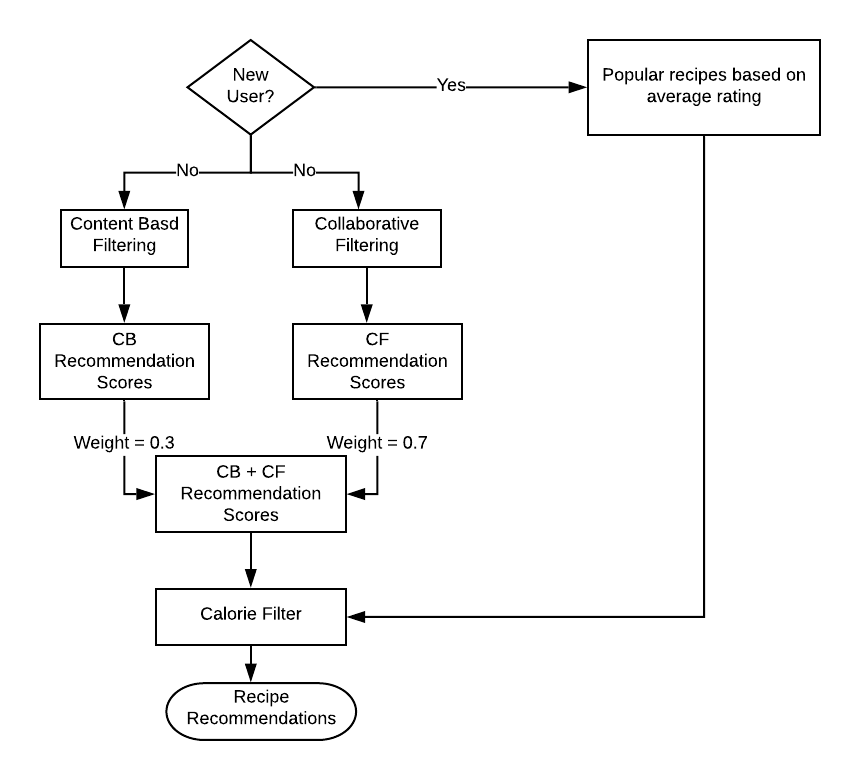
\includegraphics[width=1.0 \linewidth]{hybrid}
\caption{Hybrid Work-Flow }
\label{fig:hybrid}
\end{figure}
\end{singlespace}
\begin{itemize}
\item The system prompts to enter a user id. The existence of an entered user id is cross-verified by the system.
\item If user id exists, a content-based model that consists of ingredients, cook method and diet labels runs for this user and generates scores for relevant recipes. Once the content-based execution finishes, the collaborative filtering model runs and generates predicted ratings for all users. From this result set, predictions for a requested user are filtered out.
\item While combining scores, the weighting factor of 0.3 is applied to the content-based, and the weighting factor of 0.7 is applied to the collaborative filtering. The experiment was done considering equal weighing factors but it resulted in lower recall value of hybrid than collaborative. To improve the performance of the hybrid approach in terms of higher recall, weights were adjusted and finalized 0.3 weighing factor for content-based and 0.7 weighing factor for collaborative.
\item Scores are sorted in the descending order to get more relevant items at the top. At this point, recipes that are already rated by the user are omitted. Next, a calorie filter is applied to filter out healthy recipes.
\item Resultant set of recipes is offered as recommendations to the user.
\item If entered user id does not exist in the system, the system prompts to enter user details such as \lq{}height in inches\rq{}, \lq{}weight in lbs\rq{}, \lq{}age\rq{}, \lq{}gender\rq{} and \lq{}activity\rq{} option. The user's BMR and calorie intake per dish are calculated as discussed in the \nameref{sec:user_info}.
\item Here, the user's information goes through a popularity-based algorithm. This model finds the most popular recipes by considering the average rating for recipes and the maximum number of ratings per recipe. A list of these recipes is then sorted in descending order and filtered out by comparing recipe calories that are less than or equal to the user's calorie requirements. The resultant set of recipes is further categorized into diet labels and represented as recommendations to the user.
\item System provides an option to give feedback for a recipe in the form of ratings. The user can enter a recipe name along with its rating. This feedback is saved for future model generation and recipe recommendation for this new user.
\end{itemize}
